\documentclass[12pt,a4paper]{article}
\synctex=1
\usepackage[utf8]{inputenc}
\usepackage[margin=1cm]{geometry}
\usepackage{graphicx}
%\usepackage{verbatim}
\usepackage{listings}
\usepackage{textcomp}
\usepackage{courier}
\usepackage{libertine}
\usepackage{pgfornament}
\usepackage{eso-pic}
\usepackage[hangul]{kotex}
\linespread{1.3}

\title{
	\centering
	\pgfornament[width=12cm,color=teal]{84}\\
	\vspace{1cm}
	\fontsize{50}{50} \selectfont {객체 지향 언어 및 실습}\\
		\pgfornament[width=12cm,color=teal]{88}\\
	\vfill}
\author{
	\LARGE
	\begin{tabular}{rl}
		\hline
		학번 : & 2016110056\\ 
		학과 : & 불교학부 \\
		이름 : & 박승원\\
		날짜 : & \today\\
		\hline
	\end{tabular}\vspace{2cm}
	\\

\includegraphics[width=0.5\textwidth]{logo.jpg}
	}
\date{}


\begin{document}
\maketitle
\pagenumbering{gobble}
\noindent
\lstset{language=java, columns=flexible, tabsize=4, frame=shadowbox, showstringspaces=false, breaklines=true, upquote=true, basicstyle=\normalsize}

\includegraphics[page=2, width=0.95\textwidth]{21.pdf}
\lstinputlisting{problem1.java}
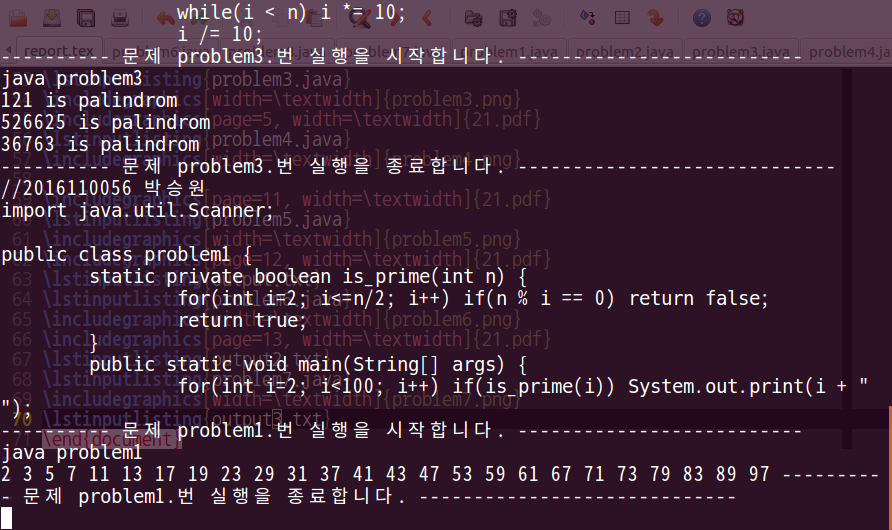
\includegraphics[width=\textwidth]{problem1.png}
\includegraphics[page=3, width=0.95\textwidth]{21.pdf}
\lstinputlisting{problem2.java}
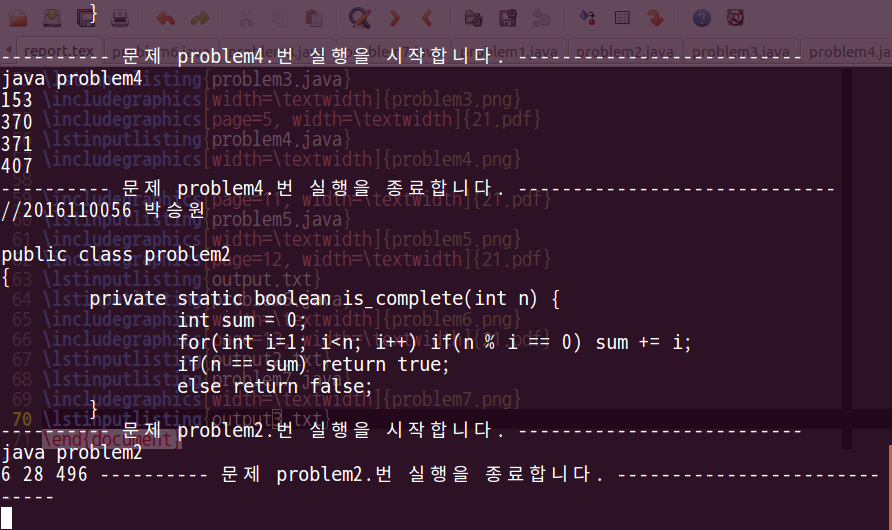
\includegraphics[width=\textwidth]{problem2.png}

\includegraphics[page=4, width=\textwidth]{21.pdf}
\lstinputlisting{problem3.java}
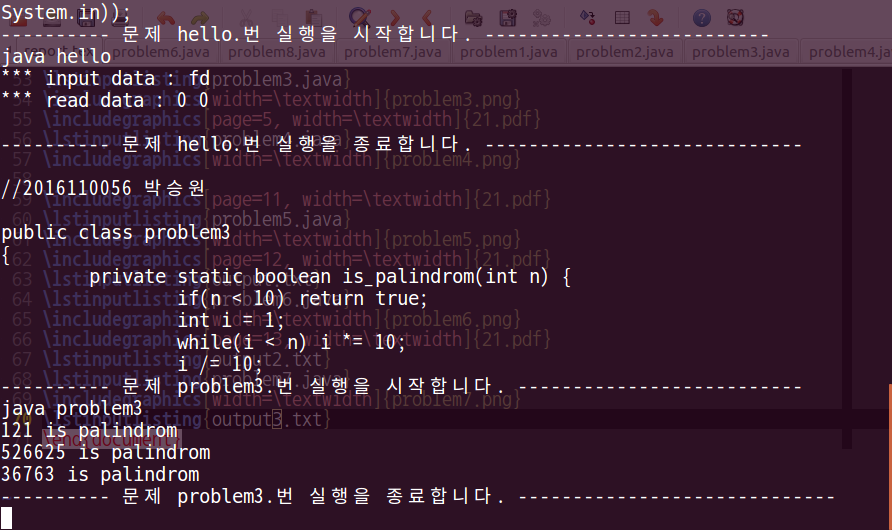
\includegraphics[width=\textwidth]{problem3.png}
\includegraphics[page=5, width=\textwidth]{21.pdf}
\lstinputlisting{problem4.java}
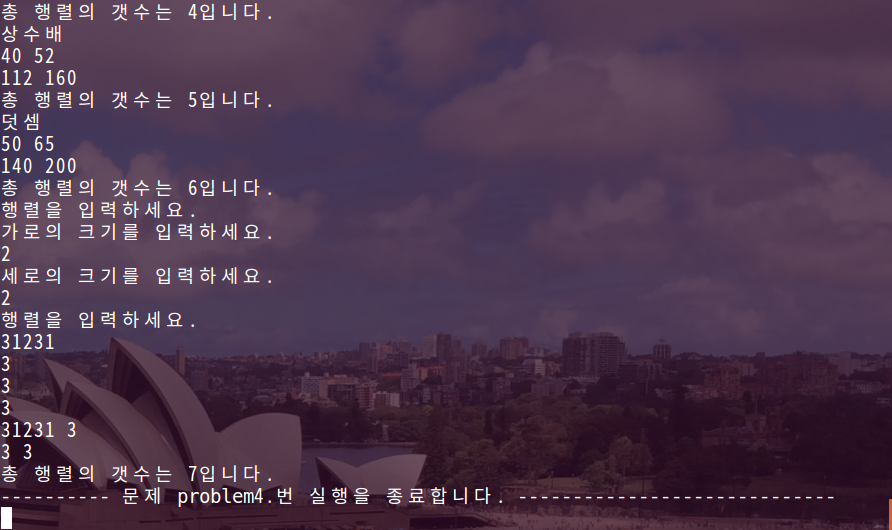
\includegraphics[width=\textwidth]{problem4.png}

\includegraphics[page=11, width=\textwidth]{21.pdf}
\lstinputlisting{problem5.java}
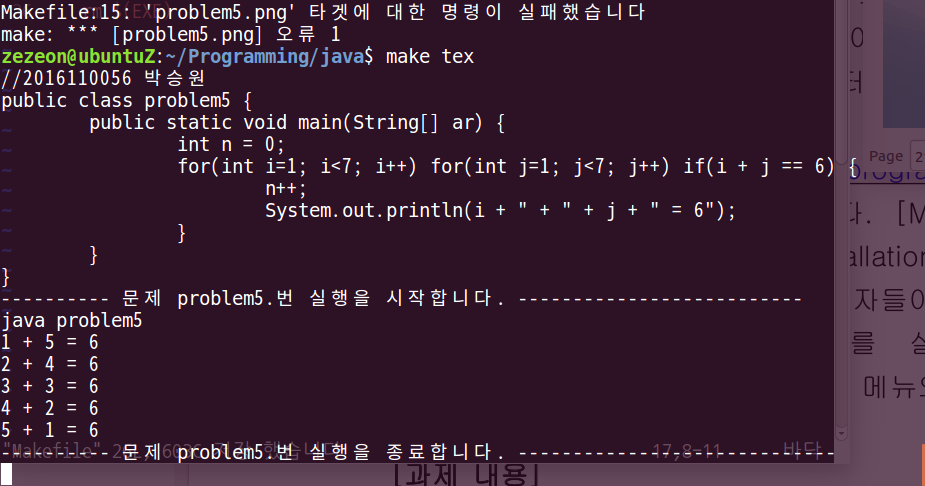
\includegraphics[width=\textwidth]{problem5.png}
\lstinputlisting{output.txt}
\includegraphics[page=12, width=\textwidth]{21.pdf}
\lstinputlisting{problem6.java}
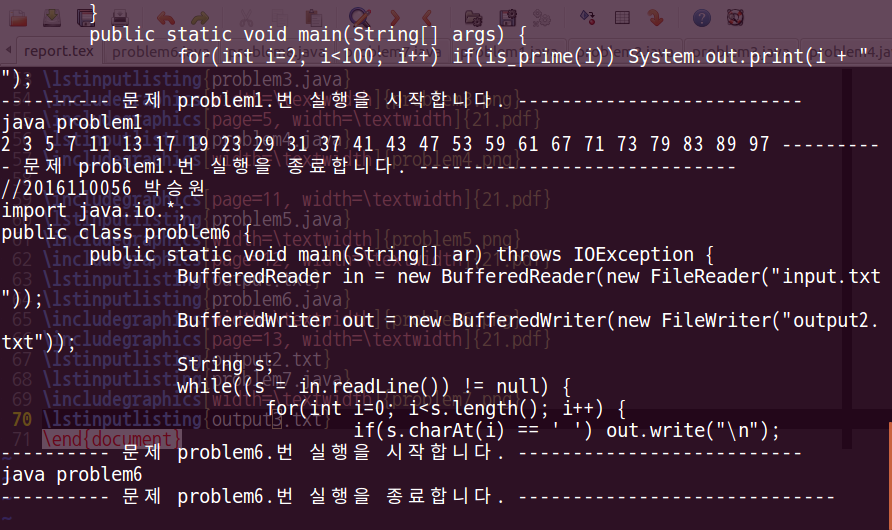
\includegraphics[width=\textwidth]{problem6.png}
\lstinputlisting{output2.txt}
\includegraphics[page=13, width=\textwidth]{21.pdf}
\lstinputlisting{problem7.java}
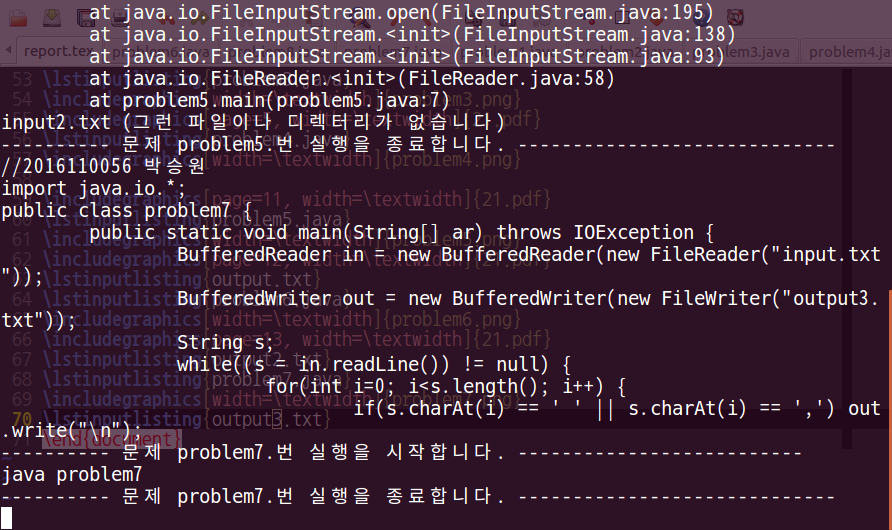
\includegraphics[width=\textwidth]{problem7.png}
\lstinputlisting{output3.txt}
\end{document}
